\documentclass[convert={density=1200,size=1080x800,outext=.svg}, tikz]{standalone}
\usetikzlibrary{matrix}
\usetikzlibrary{angles, quotes}
% \usetikzlibrary{arrows.meta}
\begin{document}
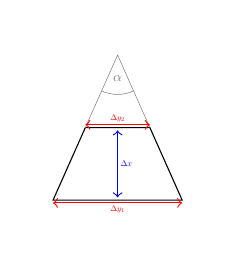
\begin{tikzpicture}

  \matrix (grid) [matrix of nodes, transparent=1]
  {
    8 & 8 & 1 & 6 & 6 \\
    3 & 3 & 5 & 7 & 7 \\
    4 & 4 & 9 & 2 & 2 \\
    4 & 4 & 9 & 2 & 2 \\
    4 & 4 & 9 & 2 & 2 \\
  };

  % runway outline
  \draw (grid-5-1.center)
  to (grid-3-2.center)
  to (grid-3-4.center)
  to (grid-5-5.center)
  to cycle;


  % runway extensions
  \draw[gray, very thin]
  (grid-3-2.center) coordinate (A) to
  (grid-1-3.center) coordinate (B) to
  (grid-3-4.center) coordinate (C)
  pic ["$\alpha$"scale=0.5, draw, solid] {angle};
  % \draw[gray, dashed, very thin, shorten <=1pt] (grid-3-4.center) to (grid-1-3.center);


  % alongtrack distance
  \draw[blue, <->, shorten >=1pt, shorten <=1pt] (grid-5-3.center) to
    node[right, scale=0.3] {$\Delta x$}
    (grid-3-3.center);

  % crosstrack distance near and far
  \draw[red, <->]
    ([yshift=-1pt]grid-5-1.center) to
    node[below, scale=0.3] {$\Delta y_{1}$}
    ([yshift=-1pt]grid-5-5.center);
    \draw[red, <->] ( [yshift=+1pt]grid-3-2.center) to
        node[above, scale=0.3] {$\Delta y_{2}$}
        ([yshift=+1pt]grid-3-4.center);

\end{tikzpicture}
\end{document}
